\chapter{A simple example of chapter title with a large length}
\index{Chapter}

\begin{phrasebox}{}{Fernando Pujaico Rivera}
\label{phrasebox:2}
This box is an environment called \CommandBox{phrasebox} that helped us put phrases. 
In this cases a phrase without title.
\end{phrasebox}


The layout of this book is defined in the \CommandBox{main.tex} 
source file of this book.
\begin{highlightbox}
\begin{verbatim}
%-------------------------------------------------------------------------------
%   Color theme of book
%-------------------------------------------------------------------------------
%%----------------------------------------------------------------------------------------
%   XCOLOR
%----------------------------------------------------------------------------------------
\RequirePackage{xcolor}

%----------------------------------------------------------------------------------------
%   Ways of define colors
%----------------------------------------------------------------------------------------

%% \colorlet{LightRubineRed}{RubineRed!70}
%% \colorlet{Mycolor1}{green!10!orange}
%% \definecolor{light-gray}{gray}{0.95}
%% \definecolor{Mycolor2}{HTML}{00F9DE}
%% \definecolor{orange}{rgb}{1,0.5,0}
%% \definecolor{DarkRed}{RGB}{98,32,6}
%% \definecolor{orange}{cmyk}{0,0.5,1,0}

%----------------------------------------------------------------------------------------
%   INTERNAL, OF THIS FILE, COLOR NAMES -- PALETE OF COLORS 
%
%   Not use this variables in book content
%----------------------------------------------------------------------------------------

% Colores básicos
\definecolor{ColorScheme1}{RGB}{48,48,48}
\definecolor{ColorScheme2}{RGB}{48,48,48}
\definecolor{ColorScheme3}{RGB}{64,64,64}
\definecolor{ColorScheme4}{RGB}{120,120,120}
\definecolor{ColorScheme5}{RGB}{240,240,240}
\definecolor{ColorScheme6}{RGB}{255,255,255}

\DefineBookColorScheme{ColorScheme1}{ColorScheme2}{ColorScheme3}{ColorScheme4}{ColorScheme5}{ColorScheme6}
%----------------------------------------------------------------------------------------
%   All the next color names are OBLIGATORY.
%----------------------------------------------------------------------------------------

% Default
\colorlet{colorDefault}{black} % Define the color used for highlighting throughout the book

% Part-chapter-title
\colorlet{colorTitlePage}{ColorScheme4}
\colorlet{colorPartPageBackground}{ColorScheme4}
\colorlet{colorPartText}{colorDefault}
\colorlet{colorChapter}{colorDefault}
\colorlet{colorSection}{colorDefault}
\colorlet{colorSectionFont}{colorDefault}
\colorlet{colorSubsection}{black}
\colorlet{colorSubsectionFont}{black}

% Boxs
\colorlet{colorAttention}{ColorScheme5}
\colorlet{colorAttentionFrame}{colorDefault}
\colorlet{colorEquationBox}{ColorScheme5}
\colorlet{colorCitationBox}{ColorScheme5}
\colorlet{colorDefinition}{colorDefault}
\colorlet{colorElaboration}{ColorScheme3}
\colorlet{colorElaborationFrame}{colorDefault}
\colorlet{colorExample}{colorDefault}
\colorlet{colorExercise}{colorDefault}
\colorlet{colorPhraseBox}{colorDefault}
\colorlet{colorInformationBox}{colorDefault}
\colorlet{colorLemma}{colorDefault}
\colorlet{colorNotation}{colorDefault}
\colorlet{colorTheorem}{colorDefault}
\colorlet{colorNote}{colorDefault!10}

% Otros
\colorlet{colorLink}{ColorScheme4}
\colorlet{colorIndex}{colorDefault}

% Init pages
\colorlet{colorPatrocinio}{white}


%----------------------------------------------------------------------------------------
%   COLOR
%----------------------------------------------------------------------------------------
\RequirePackage{color}


%%----------------------------------------------------------------------------------------
%   XCOLOR
%----------------------------------------------------------------------------------------
\RequirePackage{xcolor}

%----------------------------------------------------------------------------------------
%   Ways of define colors
%----------------------------------------------------------------------------------------

%% \colorlet{LightRubineRed}{RubineRed!70}
%% \colorlet{Mycolor1}{green!10!orange}
%% \definecolor{light-gray}{gray}{0.95}
%% \definecolor{Mycolor2}{HTML}{00F9DE}
%% \definecolor{orange}{rgb}{1,0.5,0}
%% \definecolor{DarkRed}{RGB}{98,32,6}
%% \definecolor{orange}{cmyk}{0,0.5,1,0}

%----------------------------------------------------------------------------------------
%   INTERNAL, OF THIS FILE, COLOR NAMES -- PALETE OF COLORS 
%
%   Not use this variables in book content
%----------------------------------------------------------------------------------------

% Color theme
\definecolor{ColorScheme1}{RGB}{16,81,15}
\definecolor{ColorScheme2}{RGB}{217,168,91}
\definecolor{ColorScheme3}{RGB}{255,249,128}
\definecolor{ColorScheme4}{RGB}{105,46,60}
\definecolor{ColorScheme5}{RGB}{182,106,70}
\definecolor{ColorScheme6}{RGB}{240,240,240}

\DefineBookColorScheme{ColorScheme1}{ColorScheme2}{ColorScheme3}{ColorScheme4}{ColorScheme5}{ColorScheme6}
%----------------------------------------------------------------------------------------
%   All the next color names are OBLIGATORY.
%----------------------------------------------------------------------------------------

% Default
\colorlet{colorDefault}{ColorScheme1} % Define the color used for highlighting throughout the book

% Part-chapter-title
\colorlet{colorTitlePage}{ColorScheme4}
\colorlet{colorPartPageBackground}{ColorScheme5!50!black}
\colorlet{colorPartText}{colorDefault}
\colorlet{colorChapter}{colorDefault}
\colorlet{colorSection}{colorDefault}
\colorlet{colorSectionFont}{colorDefault}
\colorlet{colorSubsection}{black}
\colorlet{colorSubsectionFont}{black}

% Boxs
\colorlet{colorAttention}{ColorScheme3}
\colorlet{colorAttentionFrame}{colorDefault}
\colorlet{colorEquationBox}{ColorScheme6}
\colorlet{colorCitationBox}{ColorScheme6}
\colorlet{colorDefinition}{colorDefault}
\colorlet{colorElaboration}{colorDefault}
\colorlet{colorElaborationFrame}{colorDefault}
\colorlet{colorExample}{colorDefault}
\colorlet{colorExercise}{colorDefault}
\colorlet{colorPhraseBox}{colorDefault}
\colorlet{colorInformationBox}{colorDefault}
\colorlet{colorLemma}{colorDefault}
\colorlet{colorNotation}{colorDefault}
\colorlet{colorTheorem}{colorDefault}
\colorlet{colorNote}{colorDefault!10}

% Otros
\colorlet{colorLink}{colorDefault}
\colorlet{colorIndex}{colorDefault}

% Init pages
\colorlet{colorPatrocinio}{ColorScheme6}


%----------------------------------------------------------------------------------------
%   COLOR
%----------------------------------------------------------------------------------------
\RequirePackage{color}


%%----------------------------------------------------------------------------------------
%   XCOLOR
%----------------------------------------------------------------------------------------
\RequirePackage{xcolor}

%----------------------------------------------------------------------------------------
%   Ways of define colors
%----------------------------------------------------------------------------------------

%% \colorlet{LightRubineRed}{RubineRed!70}
%% \colorlet{Mycolor1}{green!10!orange}
%% \definecolor{light-gray}{gray}{0.95}
%% \definecolor{Mycolor2}{HTML}{00F9DE}
%% \definecolor{orange}{rgb}{1,0.5,0}
%% \definecolor{DarkRed}{RGB}{98,32,6}
%% \definecolor{orange}{cmyk}{0,0.5,1,0}

%----------------------------------------------------------------------------------------
%   INTERNAL, OF THIS FILE, COLOR NAMES -- PALETE OF COLORS 
%
%   Not use this variables in book content
%----------------------------------------------------------------------------------------

% Color theme
\definecolor{ColorScheme1}{RGB}{43,79,96}
\definecolor{ColorScheme2}{RGB}{189,199,201}
\definecolor{ColorScheme3}{RGB}{234,211,203}
\definecolor{ColorScheme4}{RGB}{132,84,96}
\definecolor{ColorScheme5}{RGB}{120,120,120}
\definecolor{ColorScheme6}{RGB}{240,240,240}

\DefineBookColorScheme{ColorScheme1}{ColorScheme2}{ColorScheme3}{ColorScheme4}{ColorScheme5}{ColorScheme6}
%----------------------------------------------------------------------------------------
%   All the next color names are OBLIGATORY.
%----------------------------------------------------------------------------------------

% Default
\colorlet{colorDefault}{ColorScheme1} % Define the color used for highlighting throughout the book

% Part-chapter-title
\colorlet{colorTitlePage}{ColorScheme4}
\colorlet{colorPartPageBackground}{ColorScheme5!50!black}
\colorlet{colorPartText}{colorDefault}
\colorlet{colorChapter}{colorDefault}
\colorlet{colorSection}{colorDefault}
\colorlet{colorSectionFont}{colorDefault}
\colorlet{colorSubsection}{black}
\colorlet{colorSubsectionFont}{black}

% Boxs
\colorlet{colorAttention}{ColorScheme3}
\colorlet{colorAttentionFrame}{colorDefault}
\colorlet{colorEquationBox}{ColorScheme2!50}
\colorlet{colorCitationBox}{ColorScheme2!50}
\colorlet{colorDefinition}{ColorScheme4}
\colorlet{colorElaboration}{ColorScheme4}
\colorlet{colorElaborationFrame}{colorDefault}
\colorlet{colorExample}{ColorScheme4}
\colorlet{colorExercise}{ColorScheme4}
\colorlet{colorPhraseBox}{ColorScheme2}
\colorlet{colorInformationBox}{ColorScheme4}
\colorlet{colorLemma}{ColorScheme4}
\colorlet{colorNotation}{ColorScheme4}
\colorlet{colorTheorem}{ColorScheme4}
\colorlet{colorNote}{ColorScheme4!10}

% Otros
\colorlet{colorLink}{ColorScheme4}
\colorlet{colorIndexBackground}{colorDefault}
\colorlet{colorIndexText}{white}
\colorlet{colorHeader}{colorDefault}
\colorlet{colorFooter}{colorDefault}
\colorlet{colorTableBackground}{colorDefault!10}
\colorlet{colorTableLine}{white}
\colorlet{colorEnumerateBackground}{colorDefault}
\colorlet{colorEnumerateFont}{white}

% Init pages
\colorlet{colorPatrocinio}{ColorScheme2!50}


%----------------------------------------------------------------------------------------
%   COLOR
%----------------------------------------------------------------------------------------
\RequirePackage{color}


%%----------------------------------------------------------------------------------------
%   XCOLOR
%----------------------------------------------------------------------------------------
\RequirePackage{xcolor}

%----------------------------------------------------------------------------------------
%   Ways of define colors
%----------------------------------------------------------------------------------------

%% \colorlet{LightRubineRed}{RubineRed!70}
%% \colorlet{Mycolor1}{green!10!orange}
%% \definecolor{light-gray}{gray}{0.95}
%% \definecolor{Mycolor2}{HTML}{00F9DE}
%% \definecolor{orange}{rgb}{1,0.5,0}
%% \definecolor{DarkRed}{RGB}{98,32,6}
%% \definecolor{orange}{cmyk}{0,0.5,1,0}

%----------------------------------------------------------------------------------------
%   INTERNAL, OF THIS FILE, COLOR NAMES -- PALETE OF COLORS 
%
%   Not use this variables in book content
%----------------------------------------------------------------------------------------

% Color theme
\definecolor{ColorScheme1}{RGB}{22,75,89}
\definecolor{ColorScheme2}{RGB}{242,228,215}
\definecolor{ColorScheme3}{RGB}{255,184,118}
\definecolor{ColorScheme4}{RGB}{77,122,99}
\definecolor{ColorScheme5}{RGB}{120,120,120}
\definecolor{ColorScheme6}{RGB}{240,240,240}

\DefineBookColorScheme{ColorScheme1}{ColorScheme2}{ColorScheme3}{ColorScheme4}{ColorScheme5}{ColorScheme6}
%----------------------------------------------------------------------------------------
%   All the next color names are OBLIGATORY.
%----------------------------------------------------------------------------------------

% Default
\colorlet{colorDefault}{ColorScheme1} % Define the color used for highlighting throughout the book

% Part-chapter-title
\colorlet{colorTitlePage}{ColorScheme4}
\colorlet{colorPartPageBackground}{ColorScheme5!50!black}
\colorlet{colorPartText}{colorDefault}
\colorlet{colorChapter}{colorDefault}
\colorlet{colorSection}{colorDefault}
\colorlet{colorSectionFont}{colorDefault}
\colorlet{colorSubsection}{black}
\colorlet{colorSubsectionFont}{black}

% Boxs
\colorlet{colorAttention}{ColorScheme3}
\colorlet{colorAttentionFrame}{colorDefault}
\colorlet{colorEquationBox}{ColorScheme2!50}
\colorlet{colorCitationBox}{ColorScheme2!50}
\colorlet{colorDefinition}{ColorScheme4}
\colorlet{colorElaboration}{ColorScheme4}
\colorlet{colorElaborationFrame}{colorDefault}
\colorlet{colorExample}{ColorScheme4}
\colorlet{colorExercise}{ColorScheme4}
\colorlet{colorPhraseBox}{ColorScheme2}
\colorlet{colorInformationBox}{ColorScheme4}
\colorlet{colorLemma}{ColorScheme4}
\colorlet{colorNotation}{ColorScheme4}
\colorlet{colorTheorem}{ColorScheme4}
\colorlet{colorNote}{ColorScheme4!10}

% Otros
\colorlet{colorLink}{ColorScheme4}
\colorlet{colorIndexBackground}{colorDefault}
\colorlet{colorIndexText}{white}
\colorlet{colorHeader}{colorDefault}
\colorlet{colorFooter}{colorDefault}
\colorlet{colorTableBackground}{colorDefault!10}
\colorlet{colorTableLine}{white}
\colorlet{colorEnumerateBackground}{colorDefault}
\colorlet{colorEnumerateFont}{white}
% Init pages
\colorlet{colorPatrocinio}{ColorScheme2!50}


%----------------------------------------------------------------------------------------
%   COLOR
%----------------------------------------------------------------------------------------
\RequirePackage{color}


%%----------------------------------------------------------------------------------------
%   XCOLOR
%----------------------------------------------------------------------------------------
\RequirePackage{xcolor}

%----------------------------------------------------------------------------------------
%   Ways of define colors
%----------------------------------------------------------------------------------------

%% \colorlet{LightRubineRed}{RubineRed!70}
%% \colorlet{Mycolor1}{green!10!orange}
%% \definecolor{light-gray}{gray}{0.95}
%% \definecolor{Mycolor2}{HTML}{00F9DE}
%% \definecolor{orange}{rgb}{1,0.5,0}
%% \definecolor{DarkRed}{RGB}{98,32,6}
%% \definecolor{orange}{cmyk}{0,0.5,1,0}

%----------------------------------------------------------------------------------------
%   INTERNAL, OF THIS FILE, COLOR NAMES -- PALETE OF COLORS 
%
%   Not use this variables in book content
%----------------------------------------------------------------------------------------

% Color theme
\definecolor{ColorScheme1}{RGB}{72,24,8}
\definecolor{ColorScheme2}{RGB}{193,170,147}
\definecolor{ColorScheme3}{RGB}{221,165,47}
\definecolor{ColorScheme4}{RGB}{142,11,16}
\definecolor{ColorScheme5}{RGB}{111,59,23}
\definecolor{ColorScheme6}{RGB}{240,240,240}

\DefineBookColorScheme{ColorScheme1}{ColorScheme2}{ColorScheme3}{ColorScheme4}{ColorScheme5}{ColorScheme6}
%----------------------------------------------------------------------------------------
%   All the next color names are OBLIGATORY.
%----------------------------------------------------------------------------------------

% Default
\colorlet{colorDefault}{ColorScheme1} % Define the color used for highlighting throughout the book

% Part-chapter-title
\colorlet{colorTitlePage}{ColorScheme4}
\colorlet{colorPartPageBackground}{ColorScheme5!50!black}
\colorlet{colorPartText}{colorDefault}
\colorlet{colorChapter}{colorDefault}
\colorlet{colorSection}{colorDefault}
\colorlet{colorSectionFont}{colorDefault}
\colorlet{colorSubsection}{black}
\colorlet{colorSubsectionFont}{black}

% Boxs
\colorlet{colorAttention}{ColorScheme3!50}
\colorlet{colorAttentionFrame}{colorDefault}
\colorlet{colorEquationBox}{ColorScheme2!50}
\colorlet{colorCitationBox}{ColorScheme2!50}
\colorlet{colorDefinition}{ColorScheme4}
\colorlet{colorElaboration}{ColorScheme4}
\colorlet{colorElaborationFrame}{colorDefault}
\colorlet{colorExample}{ColorScheme4}
\colorlet{colorExercise}{ColorScheme4}
\colorlet{colorPhraseBox}{ColorScheme2}
\colorlet{colorInformationBox}{ColorScheme4}
\colorlet{colorLemma}{ColorScheme4}
\colorlet{colorNotation}{ColorScheme4}
\colorlet{colorTheorem}{ColorScheme4}
\colorlet{colorNote}{ColorScheme4!10}

% Otros
\colorlet{colorLink}{ColorScheme4}
\colorlet{colorIndex}{colorDefault}

% Init pages
\colorlet{colorPatrocinio}{ColorScheme2!50}


%----------------------------------------------------------------------------------------
%   COLOR
%----------------------------------------------------------------------------------------
\RequirePackage{color}


%%----------------------------------------------------------------------------------------
%   XCOLOR
%----------------------------------------------------------------------------------------
\RequirePackage{xcolor}

%----------------------------------------------------------------------------------------
%   Ways of define colors
%----------------------------------------------------------------------------------------

%% \colorlet{LightRubineRed}{RubineRed!70}
%% \colorlet{Mycolor1}{green!10!orange}
%% \definecolor{light-gray}{gray}{0.95}
%% \definecolor{Mycolor2}{HTML}{00F9DE}
%% \definecolor{orange}{rgb}{1,0.5,0}
%% \definecolor{DarkRed}{RGB}{98,32,6}
%% \definecolor{orange}{cmyk}{0,0.5,1,0}

%----------------------------------------------------------------------------------------
%   INTERNAL, OF THIS FILE, COLOR NAMES -- PALETE OF COLORS 
%
%   Not use this variables in book content
%----------------------------------------------------------------------------------------

% Color theme
\definecolor{ColorSchemeBlue}{RGB}{74,84,174}%azul
\definecolor{ColorSchemeGreen}{RGB}{21,146,129}%verde
\definecolor{ColorSchemeYellow}{RGB}{203,201,172}%amarelo
\definecolor{ColorSchemeRed}{RGB}{190,59,47}%rojo
\definecolor{ColorSchemeGreenLow}{RGB}{186,213,133}%verde low
\definecolor{ColorSchemeBlueLow}{RGB}{95,125,182}%azul low

\DefineBookColorScheme
{ColorSchemeBlue}
{ColorSchemeGreen}
{ColorSchemeYellow}
{ColorSchemeRed}
{ColorSchemeGreenLow}
{ColorSchemeBlueLow}
%----------------------------------------------------------------------------------------
%   All the next color names are OBLIGATORY.
%----------------------------------------------------------------------------------------

% Default
\colorlet{colorDefault}{ColorSchemeBlueLow} % Define the color used for highlighting throughout the book

% Part-chapter-title
\colorlet{colorTitlePage}{ColorSchemeRed}
\colorlet{colorPartPageBackground}{ColorSchemeGreenLow!50!black}
\colorlet{colorPartText}{colorDefault}
\colorlet{colorChapter}{colorDefault}
\colorlet{colorSection}{colorDefault}
\colorlet{colorSectionFont}{colorDefault}
\colorlet{colorSubsection}{ColorSchemeRed}
\colorlet{colorSubsectionFont}{ColorSchemeRed}

% Boxs
\colorlet{colorAttention}{ColorSchemeYellow}
\colorlet{colorAttentionFrame}{colorDefault}
\colorlet{colorEquationBox}{ColorSchemeBlueLow!20}
\colorlet{colorCitationBox}{ColorSchemeBlueLow!20}
\colorlet{colorDefinition}{ColorSchemeRed}
\colorlet{colorElaboration}{ColorSchemeRed}
\colorlet{colorElaborationFrame}{colorDefault}
\colorlet{colorExample}{ColorSchemeGreen}
\colorlet{colorExercise}{ColorSchemeBlueLow}
\colorlet{colorPhraseBox}{ColorSchemeBlueLow}
\colorlet{colorInformationBox}{ColorSchemeRed}
\colorlet{colorLemma}{ColorSchemeRed}
\colorlet{colorNotation}{ColorSchemeBlueLow}
\colorlet{colorTheorem}{colorDefault}
\colorlet{colorNote}{ColorSchemeRed!10}

% Otros
\colorlet{colorLink}{ColorSchemeRed}
\colorlet{colorIndexBackground}{colorDefault}
\colorlet{colorIndexText}{white}
\colorlet{colorHeader}{colorDefault}
\colorlet{colorFooter}{colorDefault}
\colorlet{colorTableBackground}{colorDefault!10}
\colorlet{colorTableLine}{white}
\colorlet{colorEnumerateBackground}{colorDefault}
\colorlet{colorEnumerateFont}{white}

% Init pages
\colorlet{colorPatrocinio}{ColorSchemeYellow}


%----------------------------------------------------------------------------------------
%   COLOR
%----------------------------------------------------------------------------------------
\RequirePackage{color}


%----------------------------------------------------------------------------------------
%   XCOLOR
%----------------------------------------------------------------------------------------
\RequirePackage{xcolor}

%----------------------------------------------------------------------------------------
%   Ways of define colors
%----------------------------------------------------------------------------------------

%% \colorlet{LightRubineRed}{RubineRed!70}
%% \colorlet{Mycolor1}{green!10!orange}
%% \definecolor{light-gray}{gray}{0.95}
%% \definecolor{Mycolor2}{HTML}{00F9DE}
%% \definecolor{orange}{rgb}{1,0.5,0}
%% \definecolor{DarkRed}{RGB}{98,32,6}
%% \definecolor{orange}{cmyk}{0,0.5,1,0}

%----------------------------------------------------------------------------------------
%   INTERNAL, OF THIS FILE, COLOR NAMES -- PALETE OF COLORS 
%
%   Not use this variables in book content
%----------------------------------------------------------------------------------------

% Color theme
\definecolor{colorBrown}{RGB}{112,70,67}
\definecolor{colorBrownLow}{RGB}{157,120,92}
\definecolor{colorBrownVeryLow}{RGB}{192,179,137}
\definecolor{colorGreenDark}{RGB}{26,88,49}
\definecolor{colorGreenLow}{RGB}{165,199,107}
\definecolor{colorGreen}{RGB}{102,143,58}

\DefineBookColorScheme
{colorBrown}
{colorBrownLow}
{colorBrownVeryLow}
{colorGreenDark}
{colorGreen}
{colorGreenLow}
%----------------------------------------------------------------------------------------
%   All the next color names are OBLIGATORY.
%----------------------------------------------------------------------------------------

% Default
\colorlet{colorDefault}{colorGreenDark} % Define the color used for highlighting throughout the book

% Part-chapter-title
\colorlet{colorTitlePage}{colorGreenDark}
\colorlet{colorPartPageBackground}{colorGreenDark!50}
\colorlet{colorPartText}{colorBrown}
\colorlet{colorChapter}{colorGreenDark}
\colorlet{colorSection}{colorBrown}
\colorlet{colorSectionFont}{colorBrown}
\colorlet{colorSubsection}{colorBrown}
\colorlet{colorSubsectionFont}{colorBrown}

% Boxs
\colorlet{colorAttention}{colorBrownVeryLow!20}
\colorlet{colorAttentionFrame}{colorBrownLow!20}
\colorlet{colorEquationBox}{colorGreenLow!20}
\colorlet{colorCitationBox}{colorGreenLow!20}
\colorlet{colorDefinition}{colorDefault}
\colorlet{colorElaboration}{colorGreen}
\colorlet{colorElaborationFrame}{colorGreen!10}
\colorlet{colorExample}{colorGreenDark}
\colorlet{colorExercise}{colorGreen}
\colorlet{colorPhraseBox}{colorDefault}
\colorlet{colorInformationBox}{colorGreenDark}
\colorlet{colorLemma}{colorDefault}
\colorlet{colorNotation}{colorDefault}
\colorlet{colorTheorem}{colorDefault}
\colorlet{colorNote}{colorDefault!10}

% Otros
\colorlet{colorLink}{colorDefault}
\colorlet{colorIndexBackground}{colorDefault}
\colorlet{colorIndexText}{white}
\colorlet{colorHeader}{colorDefault}
\colorlet{colorFooter}{colorDefault}
\colorlet{colorTableBackground}{colorGreen!5}
\colorlet{colorTableLine}{colorDefault}
\colorlet{colorEnumerateBackground}{colorBrown}
\colorlet{colorEnumerateFont}{white}

% Init pages
\colorlet{colorPatrocinio}{colorBrownVeryLow!20}


%----------------------------------------------------------------------------------------
%   COLOR
%----------------------------------------------------------------------------------------
\RequirePackage{color}







%-------------------------------------------------------------------------------
%   Configura el paquete titlesec 
%-------------------------------------------------------------------------------

\usetikzlibrary{calc}
\def\topleft{4}

\titlespacing*{\part}{-10pt}{120pt}{-80pt}%pbk
\titleformat{\part}[display]
{\Huge\filcenter\bfseries}
{}
{30pt}
{%
\begin{tikzpicture}[overlay,remember picture]
\coordinate(ptopleft) at ($(current page.north west)+(\topleft,0)$);
\foreach \i in{0,.1,.2,.3,.5,.6,.9,1.1,1.2,1.3,1.5,1.6,1.8,1.9,2}
\draw[colorsystemdefault!70]($(ptopleft)+(\i,0)$)--+(0,-\paperheight);
\node[white,fill=colorsystemdefault,minimum size=1.5cm](A) at ($(ptopleft)+(1,-5)$){\fontsize{40pt}{0pt}\sffamily\selectfont\thepart};
\node [anchor=south,ultra thick,yshift=-1mm]at(A.north){\fontsize{40pt}{0pt}\sffamily\selectfont PARTE};
\node [fill=white,anchor=north,very thick,right=-2mm,inner sep=5mm]at($(ptopleft)+(0,-0.5\paperheight)$){\parbox{\textwidth}{\fontsize{50pt}{0pt}\sffamily\selectfont #1}};
\end{tikzpicture}
}
[]

    % titleformat de part [config-1 ..config-4]
\usepackage[
TitleColor=colorChapter,
TitleFontSize=30,
PreTitleColor=colorChapter,
PreTitleFontSize=80,
BarWidth=2cm,
BarTopColor=colorChapter!20,
BarBottomColor=colorChapter!20,
BarTextColor=colorChapter!5,
BarTextFontSize=30,
BarTextOffset=1cm,
]
{chapter-format-rightbar-text}


 % titleformat de chapter [config-1 ..config-4]

\usetikzlibrary{shapes,shadows,calc}
\usetikzlibrary{positioning,calc}



\newcommand\SecTitle[5]{%
\begin{tikzpicture}

    \node (A) [rectangle,minimum width=\textwidth, minimum height=1cm,color=white,fill=colorsystemdefault, text width=\textwidth-3cm,align=left] {\hspace{1.5cm}\parbox{\textwidth}{\huge\textbf{\textsf{#4}}}};
    \fill[fill=colorsystemdefault!80] (A.north west) -- ($(A.north west)+(1.5cm,0)$) -- ($0.5*(A.north west)-0.5*(A.north west)-(0.5*\textwidth-2.5cm,0)$)--($(A.south west)+(1.5cm,0)$)--(A.south west);
    \node [color=white](A.north west) at ($0.5*(A.north west)-0.5*(A.north west)-(0.5*\textwidth-1cm,0)$) {\Huge\textbf{\textsf{#5}}};

\end{tikzpicture}

}

\titleformat{\section}
{\normalfont}{}{0em}
{\SecTitle{east}{west}{0\paperwidth}{#1}{\thesection}}

\titleformat{name=\section,numberless}
{\normalfont}{}{0em}
{\SecTitle{east}{west}{0\paperwidth}{#1}{~}}

 % section-minimalist1, %config-4} % titleformat de section [config-1 ..config-4]

\titlespacing*{\part}{-10pt}{120pt}{-80pt}%pbk
\titleformat{\part}[frame]{\Huge\filcenter\bfseries}{ \normalfont\bf\fontsize{60pt}{0pt}\selectfont \raisebox{1.7cm}{ Part\fontfamily{put}\fontseries{b}\fontsize{60pt}{0pt}\selectfont \hspace{.2em}\thepart} }{30pt}{#1}[\filright]

 % titleformat de subsection [config-1]

%-------------------------------------------------------------------------------
%   Configura header and footer 
%-------------------------------------------------------------------------------

\titlespacing*{\part}{-10pt}{120pt}{-80pt}%pbk
\titleformat{\part}[frame]{\Huge\filcenter\bfseries}{ \normalfont\bf\fontsize{60pt}{0pt}\selectfont \raisebox{1.7cm}{ Part\fontfamily{put}\fontseries{b}\fontsize{60pt}{0pt}\selectfont \hspace{.2em}\thepart} }{30pt}{#1}[\filright]

 % format [config-1]

%-------------------------------------------------------------------------------
%   Rules macros:
%-------------------------------------------------------------------------------
%-------------------------------------------------------------------------------
%   Rules macros: \HRule{2pt}, \HTextRule{Text}
%-------------------------------------------------------------------------------
\usepackage{separator-rule} %


\newcommand{\ThematicBreak}[1]
{%
\HPgfoTextRule[
Separator=3pt,
OrnamentWidth=4cm,
OrnamentColor=colorDefault,
TextFormat=\bfseries,
TextColor=colorDefault,
BeforeSpace=0pt,
AfterSpace=0pt,
]{87}{#1}%
}
 % format [separator-1]
\usepackage[
AsteriskCount=5,
BeforeSpace=0pt,
AfterSpace=0pt,
Symbol=*
]{ornamental-break-asterisks}

 % format [config1]

%-------------------------------------------------------------------------------
%   Box environments
%-------------------------------------------------------------------------------
%----------------------------------------------------------------------------------------
% HIGHLIGHTBOX BOX
%----------------------------------------------------------------------------------------
% \begin{highlightbox}
%   text
% \end{highlightbox}

\usepackage{packages/env-highlightbox-zigzag}

\SetEnvHighlightBoxZigzagThickness{1pt}
\SetEnvHighlightBoxZigzagAmplitude{3pt}

\SetEnvHighlightBoxZigzagFrameColor{gray!60}
\SetEnvHighlightBoxZigzagBackColor{gray!10}

\SetEnvHighlightBoxZigzagBeforeSpace{1ex}
\SetEnvHighlightBoxZigzagAfterSpace{1ex}

\SetEnvHighlightBoxZigzagLeftPadding{2ex}
\SetEnvHighlightBoxZigzagRightPadding{2ex}
\SetEnvHighlightBoxZigzagTopPadding{2ex}
\SetEnvHighlightBoxZigzagBottomPadding{2ex}

 % format [tcolorbox-1]
%----------------------------------------------------------------------------------------
% NOTACAO THEOREMS
%----------------------------------------------------------------------------------------
% \begin{theorem}[Título]
%   text
% \end{theorem}
%----------------------------------------------------------------------------------------
%% Create a new counter that will follow tcolorbox's numbering

\usepackage{packages/env-box-oddtab}

\NewEnvBoxOddTabGlobal[
PreTitleName=Theorem,
CounterWith=section,
BackColor=black!3,
FrameColor=black,
TitleColor=white,
PreTitleColor=black,
BackTitleColor=colorTheorem,
TitleFont=\bfseries,
BeforeSpaceLength=4pt,
AfterSpaceLength=0pt,
ImageObject={\color{black}\ding{112}},
ImageWidthLength=4ex,
PostImageObject=\hspace{1pt}
]{theorem}{TheoremOddTabCounter}{TheoremOddTabListingExt}

\newcommand{\EnvTheoremListingExt}{TheoremOddTabListingExt}
 % format [tcolorbox-1 ... tcolorbox-3]
%----------------------------------------------------------------------------------------
% ATTENTION MESSAGE BOX
%----------------------------------------------------------------------------------------
% \begin{attentionbox}
%   text
% \end{attentionbox}

\usepackage{env-highlight-foldedcorner}

\NewEnvBoxFoldedCornerGlobal[
BackColor=colorAttention!50,
FrameColor=colorAttention!50!black,
FoldColor=colorAttention!20!black,
ThicknessLength=1pt,
LeftSkipLength=0cm,
RightSkipLength=0cm,
ArcLength=3mm,
LeftRuleLength=10mm,
LeftRuleColor=colorAttention!50,
ImageObject={
\includegraphics[width=8mm]{icons/attention1.eps}},
BeforeSpaceLength=4pt,
AfterSpaceLength=4pt,
QedSymbol={},
ShadowColor=gray,
LeftPaddingLength=0ex,
RightPaddingLength=1ex,
TopPaddingLength=1.5ex,
BottomPaddingLength=1.5ex,
Breakable=true
]{attentionbox}

\begin{comment}
%% Define before space
\newcommand{\EnvAttentionBoxBeforeSpace}{2ex}
\newcommand{\SetEnvAttentionBoxBeforeSpace}[1]{\renewcommand{\EnvAttentionBoxBeforeSpace}{#1}}%

%% Define after space
\newcommand{\EnvAttentionBoxAfterSpace}{2ex}
\newcommand{\SetEnvAttentionBoxAfterSpace}[1]{\renewcommand{\EnvAttentionBoxAfterSpace}{#1}}%


\newtcolorbox{attentionbox}[1][]{enhanced,
  before skip=\EnvAttentionBoxBeforeSpace,after skip=\EnvAttentionBoxAfterSpace,
  boxrule=0.4pt,left=12mm,right=2mm,top=1mm,bottom=1mm,
  colback=colorAttention!50,
  colframe=colorAttention!20!black,
  sharp corners,rounded corners=southeast,arc is angular,arc=3mm,
  underlay={%
    \path[fill=colorAttentionFrame!20!black] ([yshift=3mm]interior.south east)--++(-0.4,-0.1)--++(0.1,-0.2);
    \path[draw=colorAttentionFrame,shorten <=-0.05mm,shorten >=-0.05mm] ([yshift=3mm]interior.south east)--++(-0.4,-0.1)--++(0.1,-0.2);
    \path[fill=colorAttention!50,draw=none] (interior.south west) rectangle node[white]{
\includegraphics[width=8mm]{icons/attention1.eps}} ([xshift=14mm]interior.north west);
    },
  drop fuzzy shadow,#1}
\end{comment}

 % format [tcolorbox-1 ... tcolorbox-3]
%----------------------------------------------------------------------------------------
% HIGHLIGHTBOX BOX
%----------------------------------------------------------------------------------------
% \begin{highlightbox}
%   text
% \end{highlightbox}

\usepackage{packages/env-highlightbox-zigzag}

\SetEnvHighlightBoxZigzagThickness{1pt}
\SetEnvHighlightBoxZigzagAmplitude{3pt}

\SetEnvHighlightBoxZigzagFrameColor{gray!60}
\SetEnvHighlightBoxZigzagBackColor{gray!10}

\SetEnvHighlightBoxZigzagBeforeSpace{1ex}
\SetEnvHighlightBoxZigzagAfterSpace{1ex}

\SetEnvHighlightBoxZigzagLeftPadding{2ex}
\SetEnvHighlightBoxZigzagRightPadding{2ex}
\SetEnvHighlightBoxZigzagTopPadding{2ex}
\SetEnvHighlightBoxZigzagBottomPadding{2ex}

 
%----------------------------------------------------------------------------------------
% HIGHLIGHTBOX BOX
%----------------------------------------------------------------------------------------
% \begin{highlightbox}
%   text
% \end{highlightbox}

\usepackage{packages/env-highlightbox-zigzag}

\SetEnvHighlightBoxZigzagThickness{1pt}
\SetEnvHighlightBoxZigzagAmplitude{3pt}

\SetEnvHighlightBoxZigzagFrameColor{gray!60}
\SetEnvHighlightBoxZigzagBackColor{gray!10}

\SetEnvHighlightBoxZigzagBeforeSpace{1ex}
\SetEnvHighlightBoxZigzagAfterSpace{1ex}

\SetEnvHighlightBoxZigzagLeftPadding{2ex}
\SetEnvHighlightBoxZigzagRightPadding{2ex}
\SetEnvHighlightBoxZigzagTopPadding{2ex}
\SetEnvHighlightBoxZigzagBottomPadding{2ex}

 

%-------------------------------------------------------------------------------
%   Theorems environments 
%-------------------------------------------------------------------------------
%----------------------------------------------------------------------------------------
% HIGHLIGHTBOX BOX
%----------------------------------------------------------------------------------------
% \begin{highlightbox}
%   text
% \end{highlightbox}

\usepackage{packages/env-highlightbox-zigzag}

\SetEnvHighlightBoxZigzagThickness{1pt}
\SetEnvHighlightBoxZigzagAmplitude{3pt}

\SetEnvHighlightBoxZigzagFrameColor{gray!60}
\SetEnvHighlightBoxZigzagBackColor{gray!10}

\SetEnvHighlightBoxZigzagBeforeSpace{1ex}
\SetEnvHighlightBoxZigzagAfterSpace{1ex}

\SetEnvHighlightBoxZigzagLeftPadding{2ex}
\SetEnvHighlightBoxZigzagRightPadding{2ex}
\SetEnvHighlightBoxZigzagTopPadding{2ex}
\SetEnvHighlightBoxZigzagBottomPadding{2ex}


%----------------------------------------------------------------------------------------
% NOTACAO THEOREMS
%----------------------------------------------------------------------------------------
% \begin{theorem}[Título]
%   text
% \end{theorem}
%----------------------------------------------------------------------------------------
%% Create a new counter that will follow tcolorbox's numbering

\usepackage{packages/env-box-ribontab}

\NewEnvBoxRibonTabGlobal[
PreTitleName=Theorem,
PreTitleColor=colorTheorem,
CounterWith=section,
BackColor=gray!5,
FrameColor=colorTheorem,
TitleColor=white,
TitleFont=\bfseries,
LeftRuleLength=2pt,
BeforeSpaceLength=4pt,
AfterSpaceLength=0pt,
ImageObject={\color{colorTheorem}\ding{112}},
ImageWidthLength=2ex,
PostImageObject=\hspace{1ex},
QedSymbol={},
LeftPaddingLength=1ex,
RightPaddingLength=1ex,
TopPaddingLength=1ex,
BottomPaddingLength=1ex
]{theorem}{TheoremRibonTabCounter}{TheoremRibonTabListingExt}

\newcommand{\EnvTheoremListingExt}{TheoremRibonTabListingExt}
 % format [tcolorbox-1 tcolorbox-2]
%----------------------------------------------------------------------------------------
% NOTACAO THEOREMS
%----------------------------------------------------------------------------------------
% \begin{notation}[Título]
%   text
% \end{notation}
%----------------------------------------------------------------------------------------
%% Create a new counter that will follow tcolorbox's numbering

\usepackage{packages/env-box-oddtab}

\NewEnvBoxOddTabGlobal[
PreTitleName=Notation,
CounterWith=section,
BackColor=black!3,
FrameColor=colorNotation!50,
TitleColor=white,
PreTitleColor=colorNotation,
BackTitleColor=colorNotation,
TitleFont=\bfseries,
BeforeSpaceLength=4pt,
AfterSpaceLength=0pt,
ImageObject={\color{colorNotation}\ding{112}},
ImageWidthLength=4ex,
PostImageObject=\hspace{1pt}
]{notation}{NotationOddTabCounter}{NotationOddTabListingExt}

\newcommand{\EnvNotationListingExt}{NotationOddTabListingExt}

\begin{comment}
\newcounter{notation}[section]
\renewcommand*{\thenotation}{\noexpand\thesection.\noexpand\arabic{notation}}


\newcommand{\titlepath}{
  \fill[colorNotation]
  (title.south east)
  --(title.east)coordinate(A)
  to[curve to,out=90,in=0]($(A)+(-5mm,5mm)$)
      --($(title.north west)+(5mm,0mm)$)coordinate(B)
to[curve to,out=180,in=90]($(B)+(-5mm,-5mm)$)coordinate(C)
      --($(C)+(0mm,-5mm)$)
      to[curve to,out=90,in=180]($(title.south west)+(+5mm,0mm)$)coordinate(F)
      --cycle;
      \draw[colorNotation,ultra thick]
      ([yshift=.5\pgflinewidth]title.south east)--
      ([yshift=.5\pgflinewidth]title.south-|interior.east);
    }

\newcommand{\EnvNotationListingExt}{MisNotation}

\newtcolorbox[list inside=MisNotation,list type=MisNotation,auto counter,number within=section]{notation}[1][]{
  enhanced,
  %frame empty,
  detach title,
  fonttitle=\bfseries,
  title={#1},
  before upper={\addtocounter{notation}{-1}\refstepcounter{notation}\textbf{Nota\c{c}\~{a}o~\thetcbcounter\refstepcounter{notation}:}},
  breakable,
  colback=colorNotation!4,
  coltitle=white,
  attach boxed title to top left={xshift=-0mm},
  boxed title style={empty},
  underlay boxed title=\titlepath

}

%%%%%%%%%%%%%%%%%%%%%%%%%%%%%%%%%%%%%%%%%%%%%%%%%%%%%%%%%%%%%%%%%%%%%%%%%%%%%%%%
%% \TocEntryEnvTextFormat está definido en generic-macros.tex
%%%%%%%%%%%%%%%%%%%%%%%%%%%%%%%%%%%%%%%%%%%%%%%%%%%%%%%%%%%%%%%%%%%%%%%%%%%%%%%%

%% List of type %% para:  \tcblistof[\section*]{MisNotation}{Lista de frases}
\titlecontents{MisNotation}[2.00cm] %% Indentation %% left
{\TocEntryEnvTextFormat} %% Spacing and font options for sections %% above code
{\contentslabel[{\thecontentslabel}]{1.45cm}} %% Section number %% numbered-entry-format % {\thetcbcounter}%
{} %% numberless-entry-format
{\ \titlerule*[.5pc]{.}\;\color{black}\thecontentspage} %% filler-page-format {\hfill\color{black}\thecontentspage} 
[] %% separator

\makeatletter
\newcommand{\ttll@MisNotation}{-1000}
\makeatother

\end{comment}

 % format [tcolorbox-1 tcolorbox-2]
%----------------------------------------------------------------------------------------
% NOTACAO THEOREMS
%----------------------------------------------------------------------------------------
% \begin{notation}[Título]
%   text
% \end{notation}
%----------------------------------------------------------------------------------------
%% Create a new counter that will follow tcolorbox's numbering

\usepackage{packages/env-box-oddtab}

\NewEnvBoxOddTabGlobal[
PreTitleName=Notation,
CounterWith=section,
BackColor=black!3,
FrameColor=colorNotation!50,
TitleColor=white,
PreTitleColor=colorNotation,
BackTitleColor=colorNotation,
TitleFont=\bfseries,
BeforeSpaceLength=4pt,
AfterSpaceLength=0pt,
ImageObject={\color{colorNotation}\ding{112}},
ImageWidthLength=4ex,
PostImageObject=\hspace{1pt}
]{notation}{NotationOddTabCounter}{NotationOddTabListingExt}

\newcommand{\EnvNotationListingExt}{NotationOddTabListingExt}

\begin{comment}
\newcounter{notation}[section]
\renewcommand*{\thenotation}{\noexpand\thesection.\noexpand\arabic{notation}}


\newcommand{\titlepath}{
  \fill[colorNotation]
  (title.south east)
  --(title.east)coordinate(A)
  to[curve to,out=90,in=0]($(A)+(-5mm,5mm)$)
      --($(title.north west)+(5mm,0mm)$)coordinate(B)
to[curve to,out=180,in=90]($(B)+(-5mm,-5mm)$)coordinate(C)
      --($(C)+(0mm,-5mm)$)
      to[curve to,out=90,in=180]($(title.south west)+(+5mm,0mm)$)coordinate(F)
      --cycle;
      \draw[colorNotation,ultra thick]
      ([yshift=.5\pgflinewidth]title.south east)--
      ([yshift=.5\pgflinewidth]title.south-|interior.east);
    }

\newcommand{\EnvNotationListingExt}{MisNotation}

\newtcolorbox[list inside=MisNotation,list type=MisNotation,auto counter,number within=section]{notation}[1][]{
  enhanced,
  %frame empty,
  detach title,
  fonttitle=\bfseries,
  title={#1},
  before upper={\addtocounter{notation}{-1}\refstepcounter{notation}\textbf{Nota\c{c}\~{a}o~\thetcbcounter\refstepcounter{notation}:}},
  breakable,
  colback=colorNotation!4,
  coltitle=white,
  attach boxed title to top left={xshift=-0mm},
  boxed title style={empty},
  underlay boxed title=\titlepath

}

%%%%%%%%%%%%%%%%%%%%%%%%%%%%%%%%%%%%%%%%%%%%%%%%%%%%%%%%%%%%%%%%%%%%%%%%%%%%%%%%
%% \TocEntryEnvTextFormat está definido en generic-macros.tex
%%%%%%%%%%%%%%%%%%%%%%%%%%%%%%%%%%%%%%%%%%%%%%%%%%%%%%%%%%%%%%%%%%%%%%%%%%%%%%%%

%% List of type %% para:  \tcblistof[\section*]{MisNotation}{Lista de frases}
\titlecontents{MisNotation}[2.00cm] %% Indentation %% left
{\TocEntryEnvTextFormat} %% Spacing and font options for sections %% above code
{\contentslabel[{\thecontentslabel}]{1.45cm}} %% Section number %% numbered-entry-format % {\thetcbcounter}%
{} %% numberless-entry-format
{\ \titlerule*[.5pc]{.}\;\color{black}\thecontentspage} %% filler-page-format {\hfill\color{black}\thecontentspage} 
[] %% separator

\makeatletter
\newcommand{\ttll@MisNotation}{-1000}
\makeatother

\end{comment}

 % format [tcolorbox-1 tcolorbox-2]
%----------------------------------------------------------------------------------------
% HIGHLIGHTBOX BOX
%----------------------------------------------------------------------------------------
% \begin{highlightbox}
%   text
% \end{highlightbox}

\usepackage{packages/env-highlightbox-zigzag}

\SetEnvHighlightBoxZigzagThickness{1pt}
\SetEnvHighlightBoxZigzagAmplitude{3pt}

\SetEnvHighlightBoxZigzagFrameColor{gray!60}
\SetEnvHighlightBoxZigzagBackColor{gray!10}

\SetEnvHighlightBoxZigzagBeforeSpace{1ex}
\SetEnvHighlightBoxZigzagAfterSpace{1ex}

\SetEnvHighlightBoxZigzagLeftPadding{2ex}
\SetEnvHighlightBoxZigzagRightPadding{2ex}
\SetEnvHighlightBoxZigzagTopPadding{2ex}
\SetEnvHighlightBoxZigzagBottomPadding{2ex}


%----------------------------------------------------------------------------------------
% NOTACAO THEOREMS
%----------------------------------------------------------------------------------------
% \begin{notation}[Título]
%   text
% \end{notation}
%----------------------------------------------------------------------------------------
%% Create a new counter that will follow tcolorbox's numbering

\usepackage{packages/env-box-oddtab}

\NewEnvBoxOddTabGlobal[
PreTitleName=Notation,
CounterWith=section,
BackColor=black!3,
FrameColor=colorNotation!50,
TitleColor=white,
PreTitleColor=colorNotation,
BackTitleColor=colorNotation,
TitleFont=\bfseries,
BeforeSpaceLength=4pt,
AfterSpaceLength=0pt,
ImageObject={\color{colorNotation}\ding{112}},
ImageWidthLength=4ex,
PostImageObject=\hspace{1pt}
]{notation}{NotationOddTabCounter}{NotationOddTabListingExt}

\newcommand{\EnvNotationListingExt}{NotationOddTabListingExt}

\begin{comment}
\newcounter{notation}[section]
\renewcommand*{\thenotation}{\noexpand\thesection.\noexpand\arabic{notation}}


\newcommand{\titlepath}{
  \fill[colorNotation]
  (title.south east)
  --(title.east)coordinate(A)
  to[curve to,out=90,in=0]($(A)+(-5mm,5mm)$)
      --($(title.north west)+(5mm,0mm)$)coordinate(B)
to[curve to,out=180,in=90]($(B)+(-5mm,-5mm)$)coordinate(C)
      --($(C)+(0mm,-5mm)$)
      to[curve to,out=90,in=180]($(title.south west)+(+5mm,0mm)$)coordinate(F)
      --cycle;
      \draw[colorNotation,ultra thick]
      ([yshift=.5\pgflinewidth]title.south east)--
      ([yshift=.5\pgflinewidth]title.south-|interior.east);
    }

\newcommand{\EnvNotationListingExt}{MisNotation}

\newtcolorbox[list inside=MisNotation,list type=MisNotation,auto counter,number within=section]{notation}[1][]{
  enhanced,
  %frame empty,
  detach title,
  fonttitle=\bfseries,
  title={#1},
  before upper={\addtocounter{notation}{-1}\refstepcounter{notation}\textbf{Nota\c{c}\~{a}o~\thetcbcounter\refstepcounter{notation}:}},
  breakable,
  colback=colorNotation!4,
  coltitle=white,
  attach boxed title to top left={xshift=-0mm},
  boxed title style={empty},
  underlay boxed title=\titlepath

}

%%%%%%%%%%%%%%%%%%%%%%%%%%%%%%%%%%%%%%%%%%%%%%%%%%%%%%%%%%%%%%%%%%%%%%%%%%%%%%%%
%% \TocEntryEnvTextFormat está definido en generic-macros.tex
%%%%%%%%%%%%%%%%%%%%%%%%%%%%%%%%%%%%%%%%%%%%%%%%%%%%%%%%%%%%%%%%%%%%%%%%%%%%%%%%

%% List of type %% para:  \tcblistof[\section*]{MisNotation}{Lista de frases}
\titlecontents{MisNotation}[2.00cm] %% Indentation %% left
{\TocEntryEnvTextFormat} %% Spacing and font options for sections %% above code
{\contentslabel[{\thecontentslabel}]{1.45cm}} %% Section number %% numbered-entry-format % {\thetcbcounter}%
{} %% numberless-entry-format
{\ \titlerule*[.5pc]{.}\;\color{black}\thecontentspage} %% filler-page-format {\hfill\color{black}\thecontentspage} 
[] %% separator

\makeatletter
\newcommand{\ttll@MisNotation}{-1000}
\makeatother

\end{comment}

% format [tcolorbox-1 tcolorbox-2]
\input{\SourceRootPath/structure/environment/proofraw/newtheorem-1}

%-------------------------------------------------------------------------------
%   Others environments 
%-------------------------------------------------------------------------------
%----------------------------------------------------------------------------------------
% HIGHLIGHTBOX BOX
%----------------------------------------------------------------------------------------
% \begin{highlightbox}
%   text
% \end{highlightbox}

\usepackage{packages/env-highlightbox-zigzag}

\SetEnvHighlightBoxZigzagThickness{1pt}
\SetEnvHighlightBoxZigzagAmplitude{3pt}

\SetEnvHighlightBoxZigzagFrameColor{gray!60}
\SetEnvHighlightBoxZigzagBackColor{gray!10}

\SetEnvHighlightBoxZigzagBeforeSpace{1ex}
\SetEnvHighlightBoxZigzagAfterSpace{1ex}

\SetEnvHighlightBoxZigzagLeftPadding{2ex}
\SetEnvHighlightBoxZigzagRightPadding{2ex}
\SetEnvHighlightBoxZigzagTopPadding{2ex}
\SetEnvHighlightBoxZigzagBottomPadding{2ex}


%----------------------------------------------------------------------------------------
% HIGHLIGHTBOX BOX
%----------------------------------------------------------------------------------------
% \begin{highlightbox}
%   text
% \end{highlightbox}

\usepackage{packages/env-highlightbox-zigzag}

\SetEnvHighlightBoxZigzagThickness{1pt}
\SetEnvHighlightBoxZigzagAmplitude{3pt}

\SetEnvHighlightBoxZigzagFrameColor{gray!60}
\SetEnvHighlightBoxZigzagBackColor{gray!10}

\SetEnvHighlightBoxZigzagBeforeSpace{1ex}
\SetEnvHighlightBoxZigzagAfterSpace{1ex}

\SetEnvHighlightBoxZigzagLeftPadding{2ex}
\SetEnvHighlightBoxZigzagRightPadding{2ex}
\SetEnvHighlightBoxZigzagTopPadding{2ex}
\SetEnvHighlightBoxZigzagBottomPadding{2ex}


%----------------------------------------------------------------------------------------
% HIGHLIGHTBOX BOX
%----------------------------------------------------------------------------------------
% \begin{highlightbox}
%   text
% \end{highlightbox}

\usepackage{packages/env-highlightbox-zigzag}

\SetEnvHighlightBoxZigzagThickness{1pt}
\SetEnvHighlightBoxZigzagAmplitude{3pt}

\SetEnvHighlightBoxZigzagFrameColor{gray!60}
\SetEnvHighlightBoxZigzagBackColor{gray!10}

\SetEnvHighlightBoxZigzagBeforeSpace{1ex}
\SetEnvHighlightBoxZigzagAfterSpace{1ex}

\SetEnvHighlightBoxZigzagLeftPadding{2ex}
\SetEnvHighlightBoxZigzagRightPadding{2ex}
\SetEnvHighlightBoxZigzagTopPadding{2ex}
\SetEnvHighlightBoxZigzagBottomPadding{2ex}



%-------------------------------------------------------------------------------
%   Others environments 
%-------------------------------------------------------------------------------
%----------------------------------------------------------------------------------------
% HIGHLIGHTBOX BOX
%----------------------------------------------------------------------------------------
% \begin{highlightbox}
%   text
% \end{highlightbox}

\usepackage{packages/env-highlightbox-zigzag}

\SetEnvHighlightBoxZigzagThickness{1pt}
\SetEnvHighlightBoxZigzagAmplitude{3pt}

\SetEnvHighlightBoxZigzagFrameColor{gray!60}
\SetEnvHighlightBoxZigzagBackColor{gray!10}

\SetEnvHighlightBoxZigzagBeforeSpace{1ex}
\SetEnvHighlightBoxZigzagAfterSpace{1ex}

\SetEnvHighlightBoxZigzagLeftPadding{2ex}
\SetEnvHighlightBoxZigzagRightPadding{2ex}
\SetEnvHighlightBoxZigzagTopPadding{2ex}
\SetEnvHighlightBoxZigzagBottomPadding{2ex}


%----------------------------------------------------------------------------------------
% HIGHLIGHTBOX BOX
%----------------------------------------------------------------------------------------
% \begin{highlightbox}
%   text
% \end{highlightbox}

\usepackage{packages/env-highlightbox-zigzag}

\SetEnvHighlightBoxZigzagThickness{1pt}
\SetEnvHighlightBoxZigzagAmplitude{3pt}

\SetEnvHighlightBoxZigzagFrameColor{gray!60}
\SetEnvHighlightBoxZigzagBackColor{gray!10}

\SetEnvHighlightBoxZigzagBeforeSpace{1ex}
\SetEnvHighlightBoxZigzagAfterSpace{1ex}

\SetEnvHighlightBoxZigzagLeftPadding{2ex}
\SetEnvHighlightBoxZigzagRightPadding{2ex}
\SetEnvHighlightBoxZigzagTopPadding{2ex}
\SetEnvHighlightBoxZigzagBottomPadding{2ex}




%-------------------------------------------------------------------------------
%   One use environments 
%-------------------------------------------------------------------------------
%----------------------------------------------------------------------------------------
% HIGHLIGHTBOX BOX
%----------------------------------------------------------------------------------------
% \begin{highlightbox}
%   text
% \end{highlightbox}

\usepackage{packages/env-highlightbox-zigzag}

\SetEnvHighlightBoxZigzagThickness{1pt}
\SetEnvHighlightBoxZigzagAmplitude{3pt}

\SetEnvHighlightBoxZigzagFrameColor{gray!60}
\SetEnvHighlightBoxZigzagBackColor{gray!10}

\SetEnvHighlightBoxZigzagBeforeSpace{1ex}
\SetEnvHighlightBoxZigzagAfterSpace{1ex}

\SetEnvHighlightBoxZigzagLeftPadding{2ex}
\SetEnvHighlightBoxZigzagRightPadding{2ex}
\SetEnvHighlightBoxZigzagTopPadding{2ex}
\SetEnvHighlightBoxZigzagBottomPadding{2ex}


\usepackage{catalographic-card} % \CatalographicCard 


%-------------------------------------------------------------------------------
%   Configura table
%-------------------------------------------------------------------------------

\titlespacing*{\part}{-10pt}{120pt}{-80pt}%pbk
\titleformat{\part}[frame]{\Huge\filcenter\bfseries}{ \normalfont\bf\fontsize{60pt}{0pt}\selectfont \raisebox{1.7cm}{ Part\fontfamily{put}\fontseries{b}\fontsize{60pt}{0pt}\selectfont \hspace{.2em}\thepart} }{30pt}{#1}[\filright]

 % format [config-1]

%-------------------------------------------------------------------------------
%   Configura itemize
%-------------------------------------------------------------------------------

\titlespacing*{\part}{-10pt}{120pt}{-80pt}%pbk
\titleformat{\part}[frame]{\Huge\filcenter\bfseries}{ \normalfont\bf\fontsize{60pt}{0pt}\selectfont \raisebox{1.7cm}{ Part\fontfamily{put}\fontseries{b}\fontsize{60pt}{0pt}\selectfont \hspace{.2em}\thepart} }{30pt}{#1}[\filright]



\titlespacing*{\part}{-10pt}{120pt}{-80pt}%pbk
\titleformat{\part}[frame]{\Huge\filcenter\bfseries}{ \normalfont\bf\fontsize{60pt}{0pt}\selectfont \raisebox{1.7cm}{ Part\fontfamily{put}\fontseries{b}\fontsize{60pt}{0pt}\selectfont \hspace{.2em}\thepart} }{30pt}{#1}[\filright]



%-------------------------------------------------------------------------------
%   Configura el paquete titlesec 
%-------------------------------------------------------------------------------
%----------------------------------------------------------------------------------------
% Chapter text styling
\titlecontents{chapter}[1.25cm] % Indentation
{\addvspace{12pt}\large\bfseries} % Spacing and font options for chapters
{\color{colorDefault!60}\contentslabel[\Large\thecontentslabel]{1.25cm}\color{colorDefault}} % [Color left Chapter number -- NADA]
{\color{colorDefault}}  %Nada
{\color{colorDefault!60}\normalsize\;\titlerule*[.5pc]{.}\;\thecontentspage} % [Color right Page number]



%----------------------------------------------------------------------------------------
% Chapter text styling
\titlecontents{chapter}[1.25cm] % Indentation
{\addvspace{12pt}\large\bfseries} % Spacing and font options for chapters
{\color{colorDefault!60}\contentslabel[\Large\thecontentslabel]{1.25cm}\color{colorDefault}} % [Color left Chapter number -- NADA]
{\color{colorDefault}}  %Nada
{\color{colorDefault!60}\normalsize\;\titlerule*[.5pc]{.}\;\thecontentspage} % [Color right Page number]



%----------------------------------------------------------------------------------------
% Chapter text styling
\titlecontents{chapter}[1.25cm] % Indentation
{\addvspace{12pt}\large\bfseries} % Spacing and font options for chapters
{\color{colorDefault!60}\contentslabel[\Large\thecontentslabel]{1.25cm}\color{colorDefault}} % [Color left Chapter number -- NADA]
{\color{colorDefault}}  %Nada
{\color{colorDefault!60}\normalsize\;\titlerule*[.5pc]{.}\;\thecontentspage} % [Color right Page number]



%----------------------------------------------------------------------------------------
% Chapter text styling
\titlecontents{chapter}[1.25cm] % Indentation
{\addvspace{12pt}\large\bfseries} % Spacing and font options for chapters
{\color{colorDefault!60}\contentslabel[\Large\thecontentslabel]{1.25cm}\color{colorDefault}} % [Color left Chapter number -- NADA]
{\color{colorDefault}}  %Nada
{\color{colorDefault!60}\normalsize\;\titlerule*[.5pc]{.}\;\thecontentspage} % [Color right Page number]



%----------------------------------------------------------------------------------------
% Chapter text styling
\titlecontents{chapter}[1.25cm] % Indentation
{\addvspace{12pt}\large\bfseries} % Spacing and font options for chapters
{\color{colorDefault!60}\contentslabel[\Large\thecontentslabel]{1.25cm}\color{colorDefault}} % [Color left Chapter number -- NADA]
{\color{colorDefault}}  %Nada
{\color{colorDefault!60}\normalsize\;\titlerule*[.5pc]{.}\;\thecontentspage} % [Color right Page number]



%----------------------------------------------------------------------------------------
% Chapter text styling
\titlecontents{chapter}[1.25cm] % Indentation
{\addvspace{12pt}\large\bfseries} % Spacing and font options for chapters
{\color{colorDefault!60}\contentslabel[\Large\thecontentslabel]{1.25cm}\color{colorDefault}} % [Color left Chapter number -- NADA]
{\color{colorDefault}}  %Nada
{\color{colorDefault!60}\normalsize\;\titlerule*[.5pc]{.}\;\thecontentspage} % [Color right Page number]






\end{verbatim}
\end{highlightbox}
where \CommandBox{\textbackslash SourceRootPath} is the variable that represents the root path of the \CommandBox{main.tex} file.
It is interesting to note that the last box used is an environment called \CommandBox{highlightbox} that wraps a \CommandBox{verbatim} environment.


To define a chapter, we use the command \CommandBox{\textbackslash chapter\{Title name\}}. 
The template settings have modified the layout design type used in the section. 
In the following sections, we will explore ways to use the most common commands in this template.

%-------------------------------------------------------------------------------
\section{A simple example of section title with a very large length}
\index{Section}

To define a section, we use the command \CommandBox{\textbackslash section\{A simple... length\}}. 
The template settings have modified the layout design type that is used in the section.


\subsection{A simple example of subsection title with a very large length}\index{Subsection}

To define a subsection, we use the command \CommandBox{\textbackslash subsection\{A simple ...} \CommandBox{length\}}. 
The template settings have modified the layout design type used in the subsection.

\subsubsection{A simple example of subsubsection title with a very large length}
\index{Subsubsection}

To define a subsubsection, we use the command \CommandBox{\textbackslash subsubsection\{A sim-} \CommandBox{ple ... length\}}. 
The template settings have modified the layout design type used in the subsection.

\paragraph{A simple example of paragraph title with a very large length}

Below of subsubsection we have the paragraph.
To define a paragraph, we use the command \CommandBox{\textbackslash paragraph\{A simple... length\}}. 
The template settings have modified the layout design type that is used in the section.
When you need to break the flow of text, you can use \CommandBox{\textbackslash OrnamentalBreak}.

\OrnamentalBreak

Another important environment is 
\CommandBox{informationbox}, 
which can be used to display some information with a title.
In the next example, we have an instance of information from Bob.

\begin{informationbox}[Título A]
\label{informationbox:1}
This box is an environment called \CommandBox{informationbox} that helped us put informations about some topic.
\end{informationbox}

The similar way to \CommandBox{\textbackslash OrnamentalBreak}, 
the \CommandBox{\textbackslash ThematicBreak} command can be used to separate 
the flow of a text, but in this case, 
it adds a title that announces the type of information in the next text.
By example: \CommandBox{\textbackslash ThematicBreak} \CommandBox{\{A very very large text in a separator rule\}}.

\ThematicBreak{A very very large text in a separator rule}%

The layout of \CommandBox{\textbackslash ThematicBreak} command is 
defined by the template of this book.

Referencia a las Frases \ref{phrasebox:1} y \ref{phrasebox:2} 

\begin{phrasebox}{Frase title A}{Autor}
\label{phrasebox:1}
\lipsum[1][1-2] 
\end{phrasebox}

\lipsum[1][1-3] 

\begin{citationbox}
\lipsum[1][1-3] 
\end{citationbox}

\lipsum[1][1-3] 

%-------------------------------------------------------------------------------
\section{Another title}\index{Index B}

This statement requires citation \cite{book_key}; this one is more specific \cite[122]{article_key}.
\lipsum[1][1-4]
 
Referencia a la Información \ref{information:2} (siguiente)

\begin{informationbox}[Título B]
\label{information:2}
\lipsum[1][1-3]\footnote{Simple footnote example.}
\end{informationbox}

\lipsum[1] % 

\begin{attentionbox}
\label{attentionbox:a}
\lipsum[1][1-3]\footnote{Simple footnote example.}
\end{attentionbox}

\lipsum[1] % 

Referencia a la Información \ref{elaboration:3} (siguiente)

\begin{elaboration}[Título C]
\label{elaboration:3}
\lipsum[1][1-3] 
\end{elaboration}

\lipsum[1][1-3] %


Referencia a la Notacion \ref{notation:0} (siguiente)

\begin{notation}[Título C]
\label{notation:0}
\lipsum[1][1-2]
\begin{itemize}
\item \lipsum[1][1-2]
\item \lipsum[1][1-2]
\begin{itemize}
\item \lipsum[1][1-2]
\item \lipsum[1][1-2]
\end{itemize}
\end{itemize}
\end{notation}

\lipsum[1][1-3] %

Referencia a la Notacion \ref{notation:1} (siguiente)

\begin{notation}[Título C]
\label{notation:1}
\lipsum[1][1-2]
\begin{enumerate}
\item \lipsum[1][1-2]
\item \lipsum[1][1-2]
\begin{enumerate}
\item \lipsum[1][1-2]
\item \lipsum[1][1-2]
\end{enumerate}
\end{enumerate}
\end{notation}

%-------------------------------------------------------------------------------
\section{Another simple title example with a very large length}
\index{Theorem  family}

\lipsum[1][1-3].
\begin{enumerate}
\item \lipsum[1][1-2]
\item \lipsum[1][1-2]
\begin{enumerate}
\item \lipsum[1][1-2]
\item \lipsum[1][1-2]
\end{enumerate}
\end{enumerate}
\lipsum[1][1-3]. See the Theorem \ref{theo:ex1:A} and Figure \ref{fig:exemplo}.
The Figure was generated by \CommandBox{chapters/cap1/python/example.py}.

\begin{figure}[htbp] % 'htbp' é uma sugestão de posicionamento
  \centering          % Centraliza a figura
  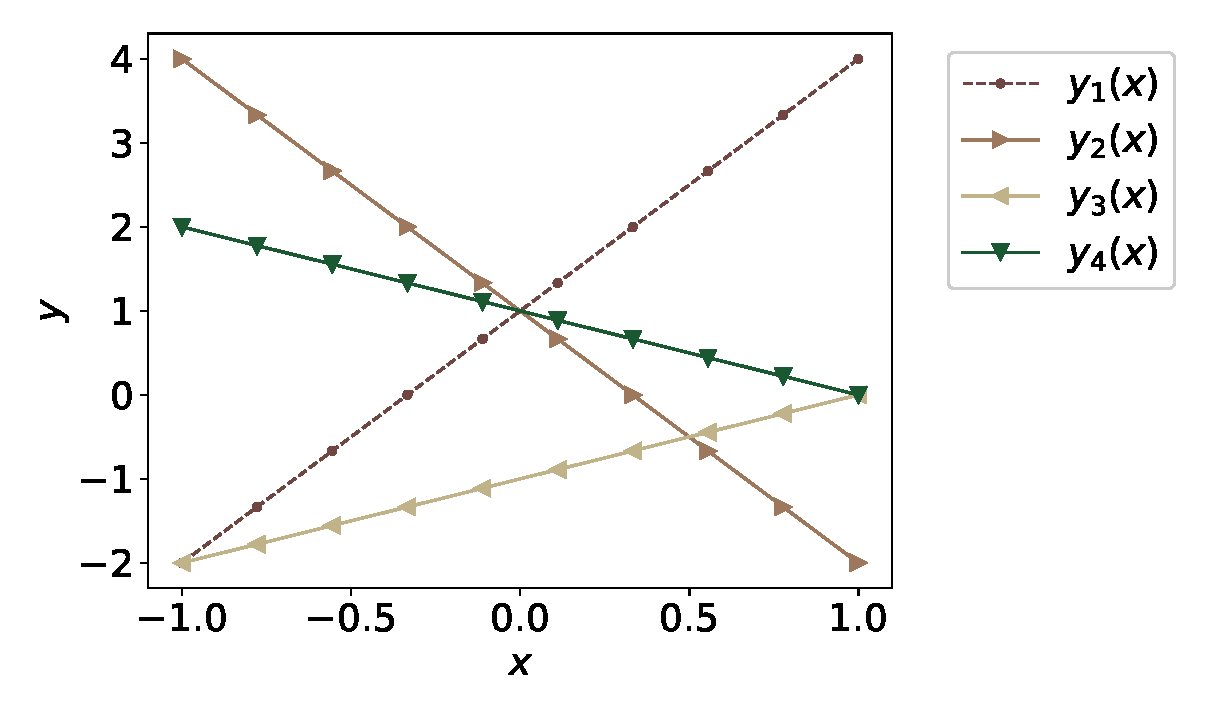
\includegraphics[width=0.75\textwidth]{chapters/cap1/python/example.eps}
  \caption{Image with the same color scheme of book} % Adiciona uma legenda
  \label{fig:exemplo} % Adiciona um rótulo para referência
\end{figure}


\begin{theorem}[Name of the theorem]
\label{theo:ex1:A}
\lipsum[1][1-3]
\begin{equation}
x^2+e^{-\frac{x^2}{2}}=1
\end{equation}
\end{theorem}

teste

\begin{proofraw}[Relative to Teorema \ref{theo:ex1:A}]
\lipsum[1][1-3]
\begin{equation}
x^2+e^{-\frac{x^2}{2}}=1
\end{equation}
\end{proofraw}
%-------------------------------------------------------------------------------
\section{Lists}\index{Lists}

\lipsum[1][1-3]\footnote{Footnote example...}.

\subsection{Numbered List}\index{Lists!Numbered List}

\begin{enumerate}
\item \lipsum[1][1-3].
\item \lipsum[1][1-3].
\item \lipsum[1][1-3].
\end{enumerate}

\subsection{Bullet Points}\index{Lists!Bullet Points}

\begin{itemize}
\item \lipsum[1][1-3].
\item \lipsum[1][1-3].
\item \lipsum[1][1-3].
\end{itemize}

\subsection{Descriptions and Definitions}\index{Lists!Descriptions and Definitions}

\begin{description}
\item[Name] \lipsum[1][1-3].
\item[Word] \lipsum[1][1-3].
\item[Comment] \lipsum[1][1-3].
\end{description}

